\documentclass[10pt]{beamer}
\usepackage{amsmath}
\usepackage{amssymb}
\usepackage{tikz}
\usetikzlibrary{arrows}

\usefonttheme{serif}

\begin{document}
\begin{frame}[c]
\frametitle{Iterative Diagonalization Algorithm (IDA)}
Consider a conventional trapped ion system, its potential has the following form,
\begin{equation*}
V = V_{\mathrm{trap}} + V_{\mathrm{Coulomb}}
\end{equation*}
The normal modes of the system are obtained by diagonalizing,
\begin{equation*}
A_{ij} = \frac{1}{\sqrt{m_i m_j}} \{\mathrm{Hess}[V](x^*)\}_{ij}
\end{equation*}
Note: Hessian of the conventional trap potential is diagonal. \\[10pt]
Therefore, only the Coulomb potential contributes to the off diagonal elements of $A$.
\end{frame}

\begin{frame}[c]
\frametitle{Iterative Diagonalization Algorithm (IDA)}
Consider adding optical tweezers on each ion,
\begin{align*}
\tilde{V} &= V_{\mathrm{trap}} + V_{\mathrm{Coulomb}} + V_{\mathrm{optical}} \\
\tilde{A}_{ij} &= \frac{1}{\sqrt{m_i m_j}} \{\mathrm{Hess}[\tilde{V}](\tilde{x}^*)\}_{ij}
\end{align*}
Note: Hessian of the optical tweezer potentials is diagonal. \\[10pt]
Therefore, only the Coulomb potential contributes to the off diagonal elements of $\tilde{A}$. \\[10pt]
Under the assumption that the equilibrium position does not change with the addition of the optical potentials, i.e. $x^* \approx \tilde{x}^*$,
\begin{equation*}
A_{ij} \approx \tilde{A}_{ij}, \, \forall \, i \neq j
\end{equation*}
\end{frame}

\begin{frame}[c]
\frametitle{Iterative Diagonalization Algorithm (IDA)}
Problem Statement: \\
Given a conventional trapped ion system and a target normal mode spectrum, $\omega^{\mathrm{target}}$. \\[10pt]
By introducing optical tweezers on each ion, are we able to find the powers, such that, the new trapped ion system has the target normal mode spectrum. \\[10pt]
Note: There may not exist a solution and solutions may not be unique.
\end{frame}

\begin{frame}[t]
\frametitle{Iterative Diagonalization Algorithm (IDA)}
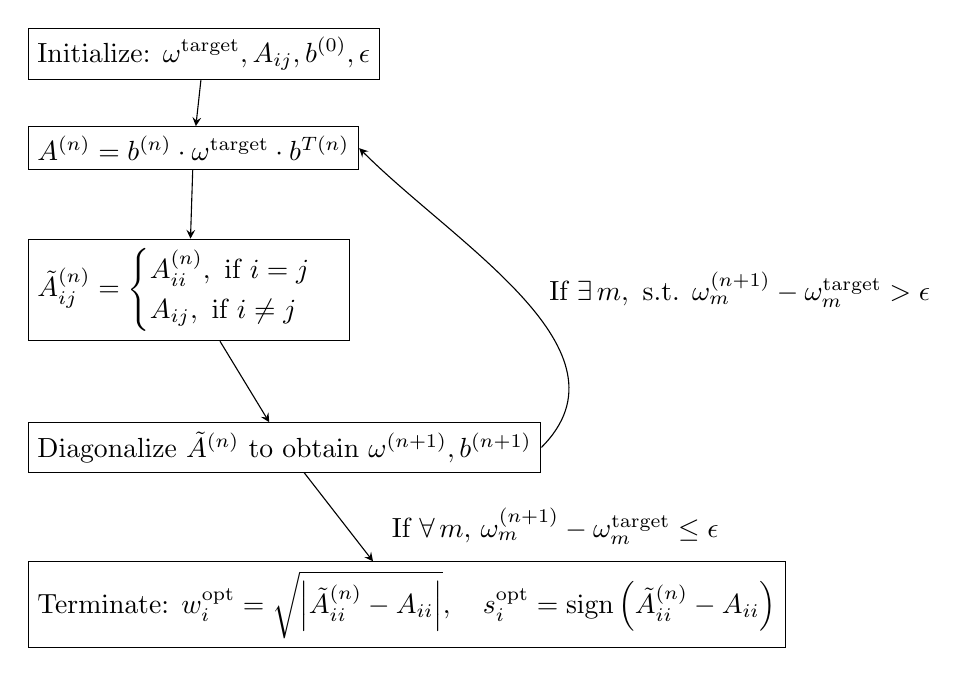
\begin{tikzpicture}
\node[draw, anchor=west] (1) at (0,0)
{Initialize: $\omega^{\mathrm{target}},A_{ij},b^{(0)}, \epsilon$};

\node[draw, anchor=west] (2) at (0,-1.2)
{$A^{(n)} = b^{(n)} \cdot \omega^{\mathrm{target}} \cdot b^{T (n)}$};

\node[draw,anchor=west] (3) at (0,-3)
{$
    \tilde{A}^{(n)}_{ij} =
    \begin{cases}
        A^{(n)}_{ii}, \text{ if } i = j \\
        A_{ij}, \text{ if } i \neq j
    \end{cases}
$} ;

\node[draw, anchor=west] (4) at (0,-5)
{Diagonalize $\tilde{A}^{(n)}$ to obtain $\omega^{(n+1)}, b^{(n+1)}$};

\node[draw, anchor=west] (5) at (0, -7)
{Terminate: $w^{\mathrm{opt}}_i = \sqrt{\left|\tilde{A}^{(n)}_{ii} - A_{ii}\right|},
\quad s^{\mathrm{opt}}_i = \mathrm{sign}\left(\tilde{A}^{(n)}_{ii} - A_{ii}\right)$};

\draw[->,>=stealth] (1) -- (2);

\draw[->,>=stealth] (2) -- (3);

\draw[->,>=stealth] (3) -- (4);

\draw[->,>=stealth] (4) -- (5);
\node[anchor=west] at (4.5,-6)
{If $\forall \, m, \, \omega^{(n+1)}_m - \omega^{\mathrm{target}}_m \leq \epsilon$};

\draw[->,>=stealth] (4.east) to [out=45,in=-45] (2.east);
\node[anchor=west] at (6.5,-3)
{If $\exists \, m, \text{ s.t. } \omega^{(n+1)}_m - \omega^{\mathrm{target}}_m > \epsilon$};
\end{tikzpicture}
\end{frame}

\begin{frame}
\frametitle{Iterative Diagonalization Algorithm (IDA)}
Problems with IDA: \\
1) There exist other points of convergence. \\[10pt]
2) Within IDA, we assumed that the equilibrium positions of the ions do not change. In actuality, the equilibrium position would change due to the optical potentials.
\end{frame}

\begin{frame}
\frametitle{Iterative Diagonalization Algorithm (IDA)}
The following condition define points of convergence for IDA, \\
$A$ and $\tilde{A}$ both have the same eigenvectors, $b$. \\
The above condition implies that,
\begin{equation*}
\omega^{\mathrm{convergence}}_m = \omega^{\mathrm{target}}_m + \delta_m
\end{equation*}
where $b_{im} \delta_m b^{T}_{mj}$ is hollow symmetric, i.e diagonal elements are 0.
Which further implies $b^2_{im}$ is not full rank and $\delta_m$ orthogonal to rows of $b^2_{im}$.

\end{frame}

\begin{frame}
\frametitle{Iterative Diagonalization Algorithm (IDA)}
Example:
\begin{align*}
&\omega^{\mathrm{target}}_m =
\begin{pmatrix}
10 & 8 & 4
\end{pmatrix} \quad
A_{i<j} =
\begin{pmatrix}
3 & 1 & 3
\end{pmatrix} \\
&b_{im} =
\frac{1}{\sqrt{6}}
\begin{pmatrix}
\sqrt{2} & \sqrt{3} & 1 \\
\sqrt{2} & 0 & -2 \\
\sqrt{2} & -\sqrt{3} & 1 \\
\end{pmatrix} \quad
A_{ij} =
\begin{pmatrix}
8 & 2 & 0 \\
2 & 6 & 2 \\
0 & 2 & 8
\end{pmatrix} \\
&\tilde{A}_{ij} =
\begin{pmatrix}
8 & 3 & 1 \\
3 & 6 & 3 \\
1 & 3 & 8
\end{pmatrix} \quad
\omega^{\mathrm{convergence}}_m =
\begin{pmatrix}
12 & 7 & 3
\end{pmatrix} \\
&\delta_m =
\begin{pmatrix}
2 & -1 & -1
\end{pmatrix} \quad
b_{im} \delta_m b^T_{mj} =
\begin{pmatrix}
0 & 1 & 1 \\
1 & 0 & 1 \\
1 & 1 & 0 \\
\end{pmatrix}
= \tilde{A}_{ij} - A_{ij} \\
&b^2_{im} =
\frac{1}{6}
\begin{pmatrix}
2 & 3 & 1 \\
2 & 0 & 4 \\
2 & 3 & 1 \\
\end{pmatrix} \quad
b^2_{im} \delta_m =
\begin{pmatrix}
0 & 0 & 0
\end{pmatrix}
\end{align*}
\end{frame}

\begin{frame}
\frametitle{Iterative Diagonalization Algorithm (IDA)}
For problem 1, using the following property of the other convergence points, $\mathrm{det}(b^2_{im})= 0$ ,we can check if our algorithm is converging to one of these points and avoid these points.
\end{frame}


\begin{frame}
\frametitle{Iterative Diagonalization Algorithm (IDA)}

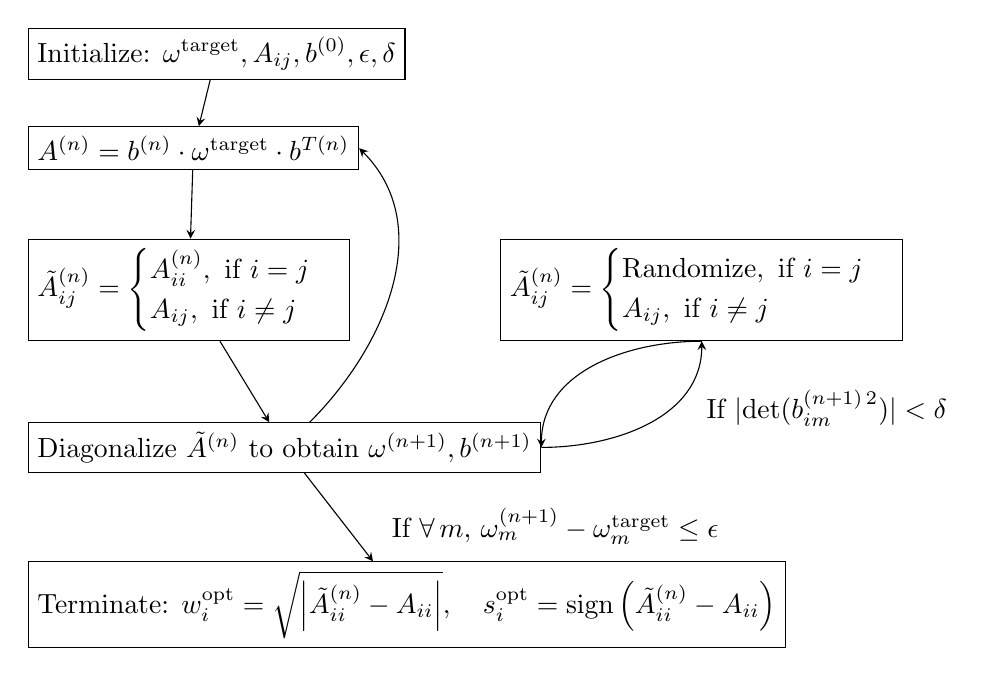
\begin{tikzpicture}
\node[draw, anchor=west] (1) at (0,0)
{Initialize: $\omega^{\mathrm{target}},A_{ij},b^{(0)}, \epsilon, \delta$};

\node[draw, anchor=west] (2) at (0,-1.2)
{$A^{(n)} = b^{(n)} \cdot \omega^{\mathrm{target}} \cdot b^{T (n)}$};

\node[draw,anchor=west] (3) at (0,-3)
{$
    \tilde{A}^{(n)}_{ij} =
    \begin{cases}
        A^{(n)}_{ii}, \text{ if } i = j \\
        A_{ij}, \text{ if } i \neq j
    \end{cases}
$};

\node[draw, anchor=west] (4) at (0,-5)
{Diagonalize $\tilde{A}^{(n)}$ to obtain $\omega^{(n+1)}, b^{(n+1)}$};

\node[draw, anchor=west] (5) at (0, -7)
{Terminate: $w^{\mathrm{opt}}_i = \sqrt{\left|\tilde{A}^{(n)}_{ii} - A_{ii}\right|},
\quad s^{\mathrm{opt}}_i = \mathrm{sign}\left(\tilde{A}^{(n)}_{ii} - A_{ii}\right)$};

\node[draw, anchor=west] (6) at (6, -3)
{$
    \tilde{A}^{(n)}_{ij} =
    \begin{cases}
        \mathrm{Randomize}, \text{ if } i = j \\
        A_{ij}, \text{ if } i \neq j
    \end{cases}
$};

\draw[->,>=stealth] (1) -- (2);

\draw[->,>=stealth] (2) -- (3);

\draw[->,>=stealth] (3) -- (4);

\draw[->,>=stealth] (4) -- (5);
\node[anchor=west] at (4.5,-6)
{If $\forall \, m, \, \omega^{(n+1)}_m - \omega^{\mathrm{target}}_m \leq \epsilon$};

\draw[->,>=stealth] (4.east) to [out=0,in=-90] (6.south);
\node[anchor=west] at (8.5,-4.5)
{If $|\mathrm{det}(b^{(n+1) \, 2}_{im})| < \delta$};

\draw[->,>=stealth] (6.south) to [out=180,in=90] (4.east);

\draw[->,>=stealth] (4) to [out=45,in=-45] (2.east);

\end{tikzpicture}
\end{frame}

\begin{frame}
\frametitle{Iterative Diagonalization Algorithm (IDA)}
For problem 2, supposing a small change in the equilibrium position due to the optical potentials, a method to compensate for the change in equilibrium position would be to perform IDA again using the new system. This could also be done iteratively. \\[10pt]

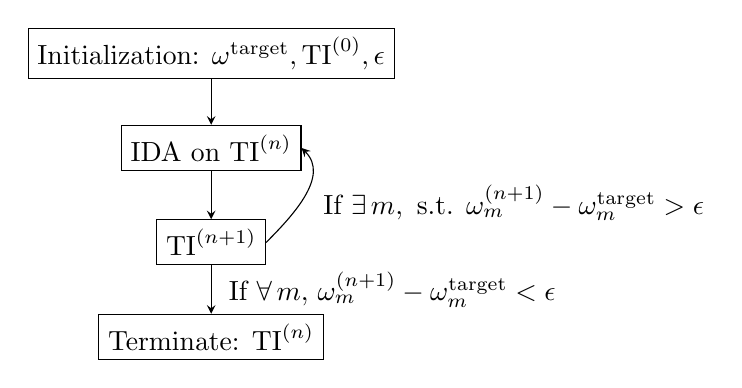
\begin{tikzpicture}
\node[draw] (1) at (0,0) {Initialization: $\omega^{\mathrm{target}},\mathrm{TI}^{(0)}, \epsilon$};

\node[draw] (2) at (0,-1.2) {IDA on $\mathrm{TI}^{(n)}$};

\node[draw] (3) at (0,-2.4) {$\mathrm{TI}^{(n+1)}$};

\node[draw] (4) at (0,-3.6) {Terminate: $\mathrm{TI}^{(n)}$};

\draw[->,>=stealth] (1) -- (2);

\draw[->,>=stealth] (2) -- (3);

\draw[->,>=stealth] (3) -- (4);
\node[anchor=west] at (0.1,-3)
{If $\forall \, m, \, \omega^{(n+1)}_m - \omega^{\mathrm{target}}_m < \epsilon$};

\draw[->,>=stealth] (3.east) to [out=45,in=-45] (2.east);
\node[anchor=west] at (1.3,-1.9)
{If $\exists \, m, \text{ s.t. } \omega^{(n+1)}_m - \omega^{\mathrm{target}}_m > \epsilon$};
\end{tikzpicture} \\[10pt]

It is yet to be determined if the above method for compensating for change in equilibrium position would work for larger changes in the equilibrium position.
\end{frame}

\begin{frame}[t]
\frametitle{Control of Normal Mode Frequencies}
\framesubtitle{Iterative Diagonalization Algorithm (IDA)}
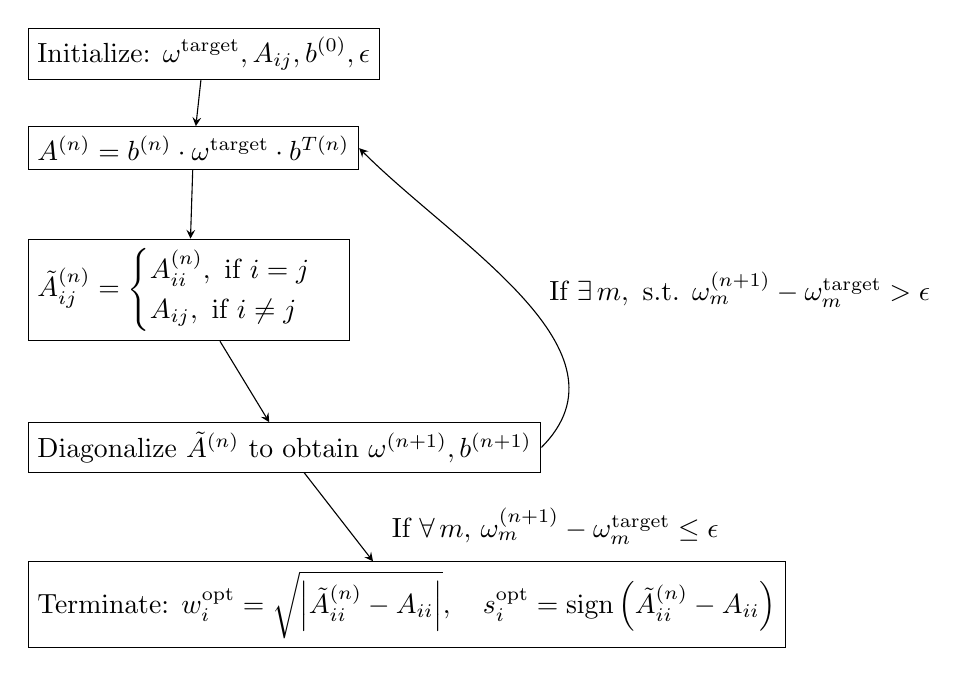
\begin{tikzpicture}
\node[draw, anchor=west] (1) at (0,0)
{Initialize: $\omega^{\mathrm{target}},A_{ij},b^{(0)}, \epsilon$};

\node[draw, anchor=west] (2) at (0,-1.2)
{$A^{(n)} = b^{(n)} \cdot \omega^{\mathrm{target}} \cdot b^{T (n)}$};

\node[draw,anchor=west] (3) at (0,-3)
{$
    \tilde{A}^{(n)}_{ij} =
    \begin{cases}
        A^{(n)}_{ii}, \text{ if } i = j \\
        A_{ij}, \text{ if } i \neq j
    \end{cases}
$} ;

\node[draw, anchor=west] (4) at (0,-5)
{Diagonalize $\tilde{A}^{(n)}$ to obtain $\omega^{(n+1)}, b^{(n+1)}$};

\node[draw, anchor=west] (5) at (0, -7)
{Terminate: $w^{\mathrm{opt}}_i = \sqrt{\left|\tilde{A}^{(n)}_{ii} - A_{ii}\right|},
\quad s^{\mathrm{opt}}_i = \mathrm{sign}\left(\tilde{A}^{(n)}_{ii} - A_{ii}\right)$};

\draw[->,>=stealth] (1) -- (2);

\draw[->,>=stealth] (2) -- (3);

\draw[->,>=stealth] (3) -- (4);

\draw[->,>=stealth] (4) -- (5);
\node[anchor=west] at (4.5,-6)
{If $\forall \, m, \, \omega^{(n+1)}_m - \omega^{\mathrm{target}}_m \leq \epsilon$};

\draw[->,>=stealth] (4.east) to [out=45,in=-45] (2.east);
\node[anchor=west] at (6.5,-3)
{If $\exists \, m, \text{ s.t. } \omega^{(n+1)}_m - \omega^{\mathrm{target}}_m > \epsilon$};
\end{tikzpicture}
\end{frame}

\begin{frame}
\frametitle{Control of Normal Mode Frequencies}
\framesubtitle{Differential Evolution (DE)}

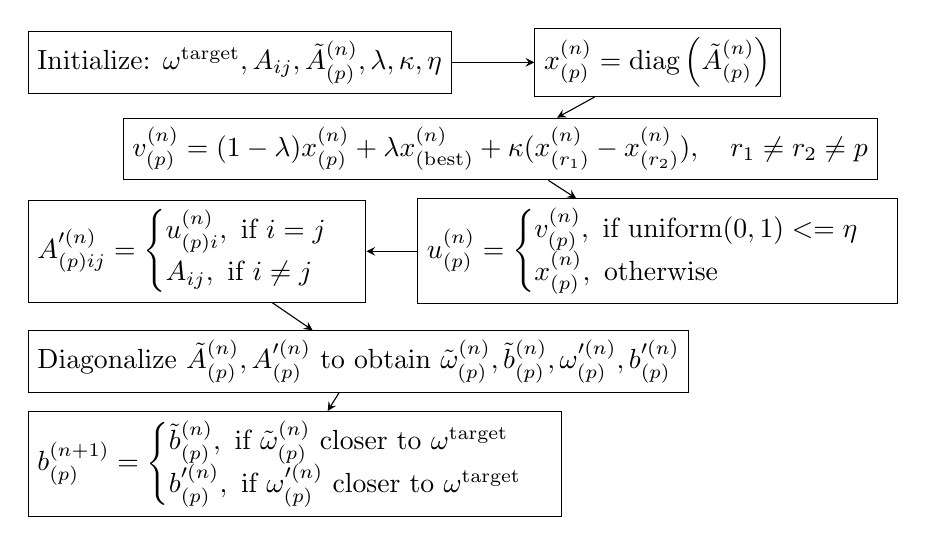
\begin{tikzpicture}
\node[draw, anchor=west] (1) at (0,-1.2)
{Initialize: $\omega^{\mathrm{target}},A_{ij},\tilde{A}^{(n)}_{(p)},\lambda,\kappa, \eta$};

\node[draw,anchor=center] (3) at (8,-1.2)
{$x^{(n)}_{(p)} = \mathrm{diag}\left(\tilde{A}^{(n)}_{(p)}\right)$};

\node[draw,anchor=center] (4) at (6,-2.3)
{$v^{(n)}_{(p)} = (1-\lambda)x^{(n)}_{(p)}+ \lambda x^{(n)}_{(\mathrm{best})} + \kappa (x^{(n)}_{(r_1)} - x^{(n)}_{(r_2)}), \quad r_1 \neq r_2 \neq p$} ;

\node[draw,anchor=center] (5) at (8,-3.6)
{$
    u^{(n)}_{(p)} =
    \begin{cases}
        v^{(n)}_{(p)}, \text{ if } \mathrm{uniform}(0,1) <= \eta \\
        x^{(n)}_{(p)}, \text{ otherwise}
    \end{cases}
$};

\node[draw, anchor=west] (6) at (0, -3.6)
{$
    A'^{(n)}_{(p)ij} =
    \begin{cases}
        u^{(n)}_{(p)i}, \text{ if } i = j \\
        A_{ij}, \text{ if } i \neq j
    \end{cases}
$};

\node[draw, anchor=west] (7) at (0,-5)
{Diagonalize $\tilde{A}^{(n)}_{(p)}, A'^{(n)}_{(p)}$ to obtain $\tilde{\omega}^{(n)}_{(p)}, \tilde{b}^{(n)}_{(p)},\omega'^{(n)}_{(p)}, b'^{(n)}_{(p)}$};

\node[draw, anchor=west] (9) at (0,-6.3)
{$
    b^{(n+1)}_{(p)} =
    \begin{cases}
        \tilde{b}^{(n)}_{(p)}, \text{ if } \tilde{\omega}^{(n)}_{(p)} \text{ closer to } \omega^{\mathrm{target}} \\
        b'^{(n)}_{(p)}, \text{ if } \omega'^{(n)}_{(p)} \text{ closer to } \omega^{\mathrm{target}}
    \end{cases}
$};

\draw[->,>=stealth] (1) -- (3);

\draw[->,>=stealth] (3) -- (4);

\draw[->,>=stealth] (4) -- (5);

\draw[->,>=stealth] (5) -- (6);

\draw[->,>=stealth] (6) -- (7);

\draw[->,>=stealth] (7) -- (9);

\end{tikzpicture}
\end{frame}

\begin{frame}
\frametitle{Control of Normal Mode Frequencies}
\framesubtitle{Iterative Diagonalization Algorithm (IDA) with Differential Evolution (DE)}

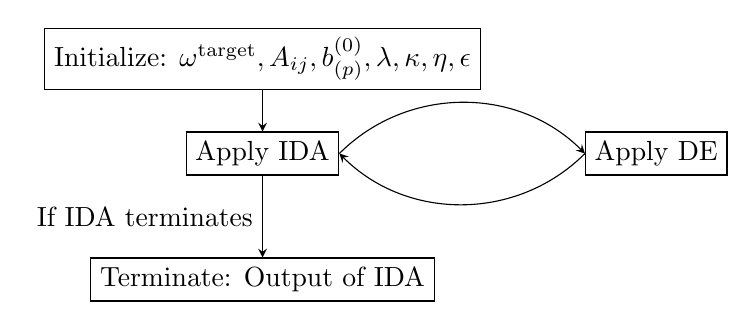
\begin{tikzpicture}
\node[draw, anchor=center] (1) at (0,0)
{Initialize: $\omega^{\mathrm{target}},A_{ij},b^{(0)}_{(p)},\lambda,\kappa, \eta, \epsilon$};

\node[draw, anchor=center] (2) at (0,-1.2)
{Apply IDA};

\node[draw, anchor=center] (3) at (5,-1.2)
{Apply DE};

\node[draw, anchor=center] (4) at (0,-2.8)
{Terminate: Output of IDA};


\draw[->,>=stealth] (1) -- (2);

\draw[->,>=stealth] (2.east) to [out=45,in=135] (3.west);

\draw[->,>=stealth] (3.west) to [out=-135,in=-45] (2.east);

\draw[->,>=stealth] (2) -- (4);
\node[anchor=east] at (0,-2)
{If IDA terminates};
\end{tikzpicture}
\end{frame}

\begin{frame}[t]
\frametitle{Control of Normal Mode Vectors}
\framesubtitle{Iterative Diagonalization Algorithm (IDA)}
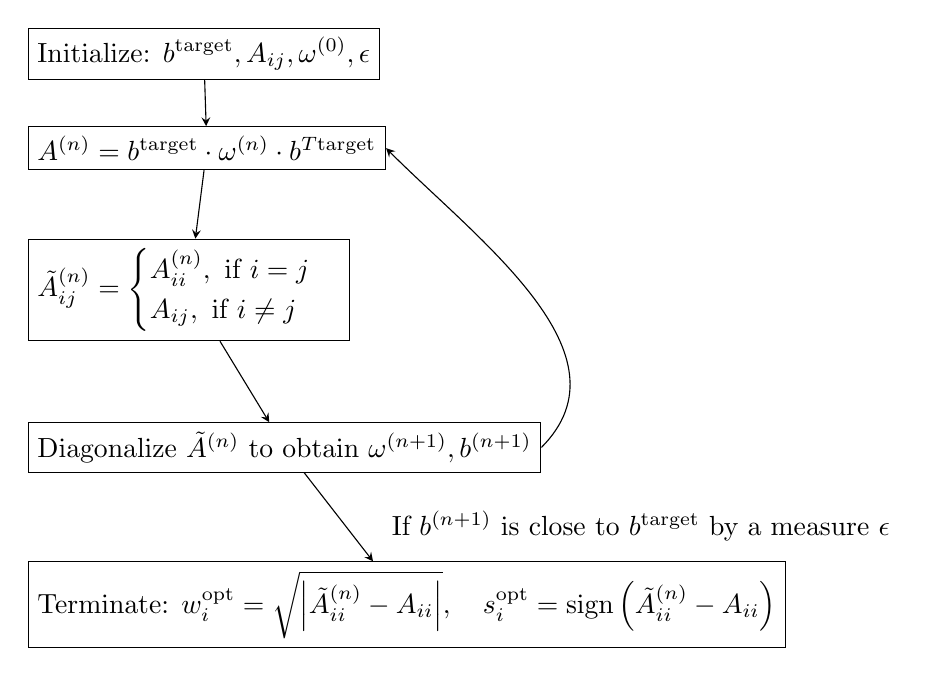
\begin{tikzpicture}
\node[draw, anchor=west] (1) at (0,0)
{Initialize: $b^{\mathrm{target}},A_{ij},\omega^{(0)}, \epsilon$};

\node[draw, anchor=west] (2) at (0,-1.2)
{$A^{(n)} = b^{\mathrm{target}} \cdot \omega^{(n)} \cdot b^{T \mathrm{target}}$};

\node[draw,anchor=west] (3) at (0,-3)
{$
    \tilde{A}^{(n)}_{ij} =
    \begin{cases}
        A^{(n)}_{ii}, \text{ if } i = j \\
        A_{ij}, \text{ if } i \neq j
    \end{cases}
$} ;

\node[draw, anchor=west] (4) at (0,-5)
{Diagonalize $\tilde{A}^{(n)}$ to obtain $\omega^{(n+1)}, b^{(n+1)}$};

\node[draw, anchor=west] (5) at (0, -7)
{Terminate: $w^{\mathrm{opt}}_i = \sqrt{\left|\tilde{A}^{(n)}_{ii} - A_{ii}\right|},
\quad s^{\mathrm{opt}}_i = \mathrm{sign}\left(\tilde{A}^{(n)}_{ii} - A_{ii}\right)$};

\draw[->,>=stealth] (1) -- (2);

\draw[->,>=stealth] (2) -- (3);

\draw[->,>=stealth] (3) -- (4);

\draw[->,>=stealth] (4) -- (5);
\node[anchor=west] at (4.5,-6)
{If $b^{(n+1)}$ is close to $b^{\mathrm{target}}$ by a measure $\epsilon$};

\draw[->,>=stealth] (4.east) to [out=45,in=-45] (2.east);
\node[anchor=west] at (6.5,-3) {};
\end{tikzpicture}
\end{frame}

\begin{frame}
\frametitle{Control of Normal Mode Vectors}
\framesubtitle{Differential Evolution (DE)}

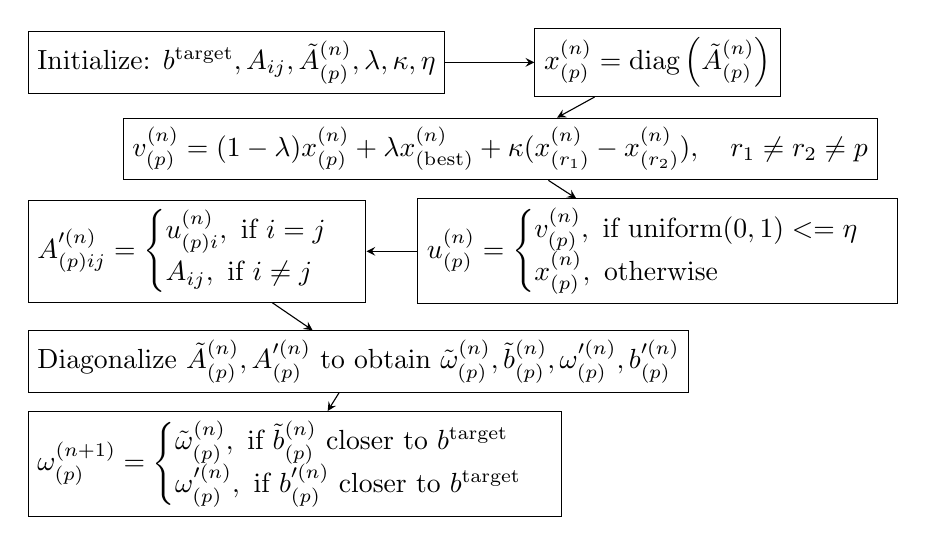
\begin{tikzpicture}
\node[draw, anchor=west] (1) at (0,-1.2)
{Initialize: $b^{\mathrm{target}},A_{ij},\tilde{A}^{(n)}_{(p)},\lambda,\kappa, \eta$};

\node[draw,anchor=center] (3) at (8,-1.2)
{$x^{(n)}_{(p)} = \mathrm{diag}\left(\tilde{A}^{(n)}_{(p)}\right)$};

\node[draw,anchor=center] (4) at (6,-2.3)
{$v^{(n)}_{(p)} = (1-\lambda)x^{(n)}_{(p)}+ \lambda x^{(n)}_{(\mathrm{best})} + \kappa (x^{(n)}_{(r_1)} - x^{(n)}_{(r_2)}), \quad r_1 \neq r_2 \neq p$} ;

\node[draw,anchor=center] (5) at (8,-3.6)
{$
    u^{(n)}_{(p)} =
    \begin{cases}
        v^{(n)}_{(p)}, \text{ if } \mathrm{uniform}(0,1) <= \eta \\
        x^{(n)}_{(p)}, \text{ otherwise}
    \end{cases}
$};

\node[draw, anchor=west] (6) at (0, -3.6)
{$
    A'^{(n)}_{(p)ij} =
    \begin{cases}
        u^{(n)}_{(p)i}, \text{ if } i = j \\
        A_{ij}, \text{ if } i \neq j
    \end{cases}
$};

\node[draw, anchor=west] (7) at (0,-5)
{Diagonalize $\tilde{A}^{(n)}_{(p)}, A'^{(n)}_{(p)}$ to obtain $\tilde{\omega}^{(n)}_{(p)}, \tilde{b}^{(n)}_{(p)},\omega'^{(n)}_{(p)}, b'^{(n)}_{(p)}$};

\node[draw, anchor=west] (9) at (0,-6.3)
{$
    \omega^{(n+1)}_{(p)} =
    \begin{cases}
        \tilde{\omega}^{(n)}_{(p)}, \text{ if } \tilde{b}^{(n)}_{(p)} \text{ closer to } b^{\mathrm{target}} \\
        \omega'^{(n)}_{(p)}, \text{ if } b'^{(n)}_{(p)} \text{ closer to } b^{\mathrm{target}}
    \end{cases}
$};

\draw[->,>=stealth] (1) -- (3);

\draw[->,>=stealth] (3) -- (4);

\draw[->,>=stealth] (4) -- (5);

\draw[->,>=stealth] (5) -- (6);

\draw[->,>=stealth] (6) -- (7);

\draw[->,>=stealth] (7) -- (9);
\end{tikzpicture}
\end{frame}

\begin{frame}
\frametitle{Control of Normal Mode Vectors}
\framesubtitle{Iterative Diagonalization Algorithm (IDA) with Differential Evolution (DE)}

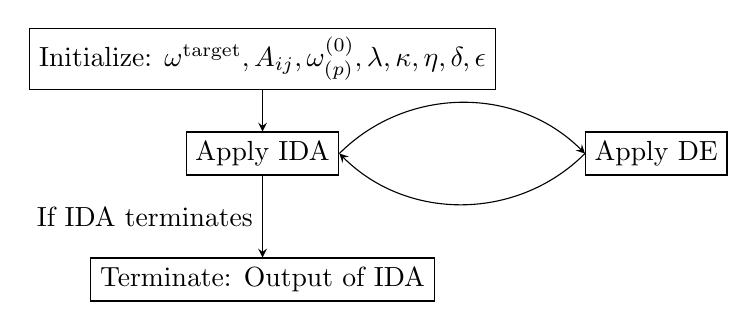
\begin{tikzpicture}
\node[draw, anchor=center] (1) at (0,0)
{Initialize: $\omega^{\mathrm{target}},A_{ij},\omega^{(0)}_{(p)},\lambda,\kappa, \eta, \delta, \epsilon$};

\node[draw, anchor=center] (2) at (0,-1.2)
{Apply IDA};

\node[draw, anchor=center] (3) at (5,-1.2)
{Apply DE};

\node[draw, anchor=center] (4) at (0,-2.8)
{Terminate: Output of IDA};


\draw[->,>=stealth] (1) -- (2);

\draw[->,>=stealth] (2.east) to [out=45,in=135] (3.west);

\draw[->,>=stealth] (3.west) to [out=-135,in=-45] (2.east);

\draw[->,>=stealth] (2) -- (4);

\node[anchor=east] at (0,-2)
{If IDA terminates};
\end{tikzpicture}
\end{frame}
\end{document}
